\documentclass[a4paper, openany]{memoir}

\usepackage[utf8]{inputenc}
\usepackage[T1]{fontenc} 
\usepackage[english]{babel}
\usepackage{amsmath}
\usepackage{amssymb}

\usepackage{booktabs}
\usepackage{fancyhdr}
\usepackage{float}
\usepackage{indentfirst}
\usepackage{graphicx}
\usepackage[linewidth=1pt]{mdframed}
\usepackage{multicol}
\usepackage{fancyvrb}

\pagestyle{fancy}
\fancyhf{}
\fancyhead[LE]{\leftmark}
\fancyhead[RO]{\rightmark}
\fancyhead[RE, LO]{PSD}
\fancyfoot[LE, RO]{\thepage}
\fancyfoot[RE, LO]{Pete Gautam}

\renewcommand{\headrulewidth}{1.5pt}

\chapterstyle{thatcher}
\setcounter{chapter}{1}

\begin{document}

\chapter{Agile Team Organisation}
\section{Agile Manifesto}
In the previous chapter, we saw that early software development methods did not consider the intrinsic complexity of a software. Schwaer and Beedle (2001) said that these methods followed a systematic approach- projects were made to fit around a pre-planned process. This does not allow us to deal with the complexity, unpredictability and the evolution of software projects. Instead, they argued that the software development process should be agile- the process should fit around the projects. A software project changes all the time, as it becomes better understood. 

This led to the proposal of the agile manifesto by software practitioners. They wanted a new approach for software development where:
\begin{itemize}
    \item the process focused on individuals and interactions rather than the processes and tools;
    \item the process focused on producing a working software rather than a comprehensive documentation of the software (as the evidence of the state of the project is more important);
    \item the process focused on customer collaboration rather than contact negotiations (so the customer could understand change as it took place);
    \item the process focused on responding to change rather than following a procedure (so that it is possible to adjust the software plan and process as the software changes).
\end{itemize}

\section{Agile Processes}
Normally, an agile team is small- it typically consists of around 3-12 developers. The team members communicate frequently, through short, structured team meetings and also informal communication. They review small deliveries of features frequently. More importantly, they communicate frequently with the customer, e.g. to review requirements and features. 

The code is maintained throughout the process, using testing, analysis, code reviews and refactoring. That is, the quality assurance stage is not a discrete phase; it is taking place all the time. There is an aim to automate the process whenever possible- this lowers the need to develop supplementary documentations for artifacts. 

There is also frequent review and change of project objectives and priorities- this is done by communicating not just with the team, but also the customer. Also, we analyse and review the software process frequently to enhance the performance. This means we are not following a predefinedd process.

Over the last 20/30 years, many agile methods have been developed, such as:
\begin{itemize}
    \item Xtreme Programming,
    \item Scrum,
    \item Lean,
    \item Feature Drive Development,
    \item Crystal clear,
    \item Kanban.
\end{itemize}
\noindent In particular, they make use of the agile practices, such as:
\begin{itemize}
    \item Test driven development,
    \item Behaviour drive development,
    \item Planning poker,
    \item Refactoring,
    \item Pair Programming,
    \item Retrospectives,
    \item Continuous integration and deployment.
\end{itemize}

Although agile development is a better way to develop software, there are many risks to it:
\begin{itemize}
    \item There could be a lack of customer engagement. Agile development aims for frequent communication with customer. So, a project might fail if the customer is not engaged.
    
    \item There might be stakeholder conflict. The agile development is based on having one true set of requirements/stakeholder. However, there are many stakeholders involved in a project, and each of which might have a conflicting requirements, for example.
    
    \item It gives rise to complex contractual arrangements. In agile development, the requirements are deliberately not set at the start of the process. So, it is difficult to allocate a budget at the start, for example.
    
    \item It is possible for the organisational memory to be lost. Typically, written documentation is used to describe why certain choices were made during the process. However, since agile development has a lower emphasis on documentation, it gets difficult to keep track of the reasons why something was done, especially as people leave and join the team.
    
    \item The code quality might get poor. We are constantly changing the code base, so the code quality might get lower and it gets difficult to maintain the code. This can be mitigated with code testing and refactoring.
    
    \item There might be poor team coordination and cohesion. The agile process is dependent on continual communication within the team.
\end{itemize}

Agile development does not mean that every agile practice should be used within a project. Each project is different, and different practices are suited for different projects. A team should decide which set of practices they should follow for a project. Also, we do not achieve flexibility within a project by changing objectives and processes without any structure- agile processes still have discipline.

\section{Scrum Development}
We will now look at an agile method- scrum development. This approach focuses on team, project and process management aspects of software development. It can be used to wrap around other practices that cover technical concerns (e.g. test-driven development and refactoring). 

\subsection{Roles}
A scrum team has two key roles:
\begin{itemize}
    \item The scrum master is a coach and mentor to the team. They help improve the software process and remove obstacles stopping the objectives being met.
    \item The product owner liaises between the software team and external stakeholders (e.g. customer, users). They try to understand the needs of the stakeholders and then communicate it with the team.
\end{itemize}
There are other roles as well, such as:
\begin{itemize}
    \item The team manager assigns tasks to developers. Some teams do not have an explicit team manager and just assign the tasks as a team.
    \item The quality assurance manager assigns code reviews and reviews test-code coverage.
    \item The toolsmith maintains the development infrastructure, e.g. version control environment and continuous integration tools.
    \item The chief architect makes key design decisions about the software.
    \item The user experience (UX) designer develops the user interface, often with the customer and the users.
    \item The developers write code.
\end{itemize}

\subsection{Scrum workflow}
In the scrum practice, work is organised into releases. A released is marked by an initial release-planning meeting. Before the first sprint, it is common to have a project-launch meeting- it sets the key objectives of the project. A release can have one or more sprints. Each sprint lasts between 1 and 3 weeks, where a team makes small changes. A sprint starts with a planning meeting (where the team can decide the objectives for the sprint) and ends with a review (where the team discusses what was achieved) and a retrospective (where the team reflects on the sprint and thinks of ways to improve the process). Stand ups and scrums may take place throughout the sprint- these may be daily or less frequent.

The workflow of a sprint is shown below:
\begin{figure}[H]
    \centering
    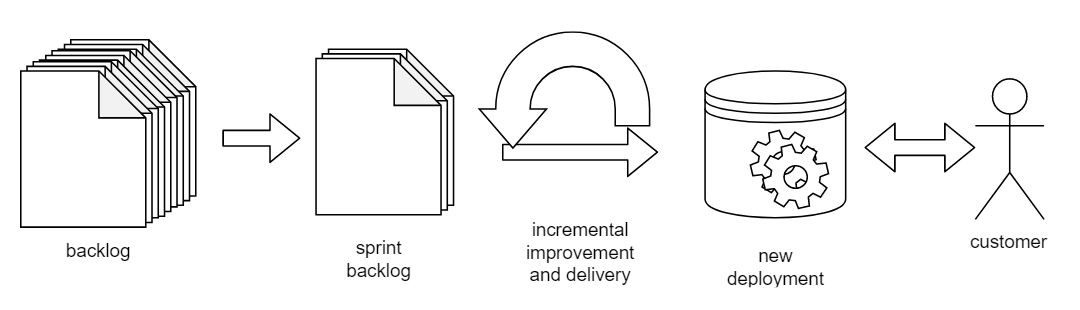
\includegraphics[scale=0.3]{src/2.1 SrcumWorkflow.png}
    \caption{The workflow of a sprint.}
\end{figure}
\noindent The process starts with reviewing the backlog. This is stuff that could be implemented during the project. Then, the sprint backlog is decided. This is a subset of all the tickets in the backlog that are to be done in the sprint. This takes into consideration the customer's priorities. The team then works on the project for some weeks, developing new code and version of the software. They then deploy the new version of code to the product environment. At the end of the sprint, the customer reviews code and gives feedback.

\subsection{Project launch meeting}
In a project launch meeting:
\begin{itemize}
    \item the team determines the major features to be delivered to the customer over a series of sprints;
    \item the team tries to understand the customer's long term objectives and identify a minimum viable product- this is a smaller set of features that allow the customer to get value out of the project;
    \item the team decides on the goals for within the course of the project;
    \item the team develops an initial set of user stories, and refines them into tasks and populates the backlog;
    \item the team triages items in the backlog to make cost estimates and assign priorities (this will change over time as the customer understands more of the project);
\end{itemize}

\subsection{Release planning meeting}
For longer projects, there will be multiple releases. Each release has many sprints. In a release planning meeting:
\begin{itemize}
    \item the team identifies high level set of features and improvements to be delivered in a release;
    \item the team creates a roadmap of milestones aligned with the customer priorities;
    \item the team populates the roadmap with key features from the backlog (we assume that these will change in sprint planning meetings, according to customer priorities).
\end{itemize}

\subsection{Sprint-planning meeting}
In a sprint-planning meeting:
\begin{itemize}
    \item the team decides on the main goals for the sprint (e.g. major new feature set, performance enhancements, bugs fixed, code improvement, etc.)  using customer feedback/requirements;
    \item the team choose tasks from the backlog that match the goals;
    \item the team ensures that the chosen issues are detailed- they have cost estimates (within the project velocity), priorities assigned, and team members assigned;
\end{itemize}
The meeting should last about 1-2 hours.

We can determine project velocity using a burn down chart, like the one shown below.
\begin{figure}[H]
    \centering
    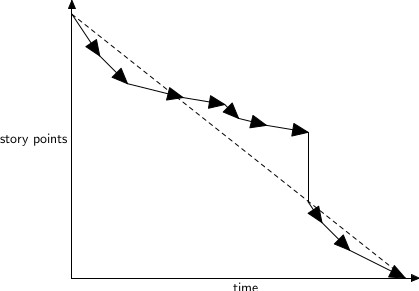
\includegraphics[scale=0.8]{src/2.2 BurnDownCharts.png}
    \caption{A burn down chart.}
\end{figure}
\noindent The dotted line shows how we expect the ideal effort to be in the project at a given time. The other line shows what it actually is- it is ahead of the project velocity at times, and sometimes behind the ideal velocity. Velocity is a useful notion used to measure the effort available within a sprint. Story points is an effort metric (other metrics include price).

\subsection{Stand-ups}
We have (daily) stand-ups to monitor team progress. It should take place at least one a week, ideally once a day. During the meeting, the scrum master asks each member:
\begin{itemize}
    \item What did you do since the last meeting?
    \item What are you doing now?
    \item Do you have any blockers?
\end{itemize}
The meeting should not last more than 10 minutes- the meeting is not to resolve the issues, but to raise them to everyone on the team. It is a good idea to document stand-ups on the wiki. It helps facilitate communication and review.

\subsection{Sprint review meeting and retrospectives}
We have sprint review meetings to review progress. It is an opportunity to gather feedback on team progress from the customer. We also have the opportunity to review the software progress in retrospectives.

During a sprint review meeting:
\begin{itemize}
    \item the team delivers and demonstrates a new version of the software that was developed over the last sprint;
    \item the team summarises their progress, and how it deviated for the plan- what additional work was completed, and which features were missed;
    \item the team explains why the team deviated from the plan;
    \item the team identifies the new features to be added to the system during the next sprint- this allows the team to gather feedback before the sprint planning meeting.
\end{itemize}

\subsection{Managing Delays}
When a team encounters a delay during a sprint, the team has many options, such as:
% TODO: Figure out which one is deadline drive and which is feature driven
\begin{itemize}
    \item The team can ask for an extension to complete the task. This delays the delivery of the software to the customer so that the feature can be completely implemented. This is risky- we do not get any feedback from the customer, and the requirements might have changed by the end of the extension.
    \item The team can reduce the feature set. In this case, the team will move some of the features to the next sprint so it can be completed later. This is more sensible in achieving goals and managing delays. The customer gets something of value delivered on time, which means that there is a chance to get feedback.
    
    \item The team can reduce resources from the project so that it can be delivered on time. For example, we can reduce the quality assurance practices. This is risky- the software might end up having some critical bugs.
\end{itemize}

Also, the team can add resources to the project for it to be delivered on time. For instance, we can add more team members. Brooks (1995) argued that due to the complex nature of software development, this is not always successful. In an ideal scenario, we would expect the following:
\begin{figure}[H]
    \centering
    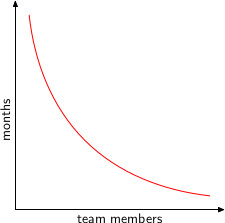
\includegraphics{src/2.3 Ideal.png}
    \caption{Team members and the amount it takes to complete a software project (in months) in an ideal setting.}
\end{figure}
\noindent So, adding more team members means that the project is completed faster. This only works if the project is partitionable. Moreover, in practice, the graph is more like the following:
\begin{figure}[H]
    \centering
    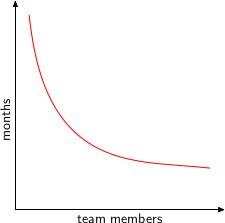
\includegraphics{src/2.4 WithTraining.png}
    \caption{Team members and the amount it takes to complete a software project (in months) in practice.}
\end{figure}
\noindent This is because adding more members is not simple- a team member requires some training. This means that there is a constant amount of time required for training each team member. In some cases, however, adding more people does not make a difference.
\begin{figure}[H]
    \centering
    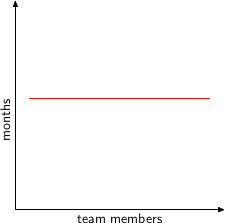
\includegraphics{src/2.5 Unpartitionable.png}
    \caption{Team members and the amount it takes to complete a software project (in months) for an unpartitionable project.}
\end{figure}
\noindent This is true for unpartitionable projects. The number of team members does not affect the length of software development. The structure of the project means that people cannot make effective contribution. Also, it is possible for us to end up with the following case for a complex software project:
\begin{figure}[H]
    \centering
    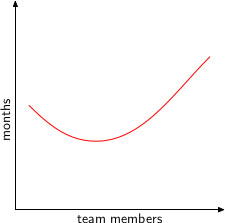
\includegraphics{src/2.6 Complex.png}
    \caption{Team members and the amount it takes to complete a software project (in months) for a complex project.}
\end{figure}
\noindent This applies to many projects. Adding more people increases time due to additional communication overhead required. This is counterproductive.

In summary, agile methods manage project risk through frequent reviews and small adjustments to project objectives and progress. It is not a discipline-free approach to software development. Instead, it requires considerable discipline to be applied effectively.
\end{document}